% !TeX root = RJwrapper.tex
\title{Working with Code environments in texor}
\author{by Abhishek Ulayil}

\maketitle

\abstract{
This is a small sample article to demonstrate usage of texor to convert code environments.
}

\section{Introduction}

Pandoc naturally converts verbatim environment easily, however the redefination of other commands such as example, example*, Sinput etc to verbatim does not work well in pandoc.

Hence \CRANpkg{texor} package uses the stream editor to search find and replace matching code environments to verbatim before pandoc touches it.

This way the the code is not lost in conversion, also a pandoc extension is used to add attributes to the markdown code using  \verb|fenced_code_attributes|

Code Environment types are well summarized in the table \ref{table:1}

\begin{table}[htbp]
\centering
\begin{tabular}{l | lllll }
 \hline
 Code Environment Type &  &  &  & & \\
 \hline
 Example          & example & example* &  & & \\
 S.series         & Sin & Sout & Sinput & Soutput & Scode \\
 Special Verbatim & boxedverbatim & &  & & \\
\hline
\end{tabular}
\caption{Code Environment support in texor}
\label{table:1}
\end{table}


\section{Environments}

\subsection{Verbatim Series}
While verbatim is naturally supported in pandoc,other extensions of verbatim environment
like boxedverbatim from moreverb package \citep{moreverb}.
% verbatim

1. verbatim :

\begin{verbatim}
print("Hello world")
\end{verbatim}


2. boxedverbatim :

\begin{boxedverbatim}
print("Hello world")
\end{boxedverbatim}


\subsection{S series}

S series code environement is defined in Rjournal.sty file.

1. Sinput :

\begin{Sinput}
print("Hello world")
\end{Sinput}


2. Soutput :

\begin{Soutput}
[1] "hello world"
\end{Soutput}


3. Sin :

\begin{Sin}
print("Hello world")
\end{Sin}


4. Sout :
\begin{Sout}
[1] "hello world"
\end{Sout}


\subsection{Example series}
Example series of code environment is defined in Rjournal.sty file.

1. example :

\begin{example}
print("Hello world")
\end{example}


2. example* :

\begin{example*}
print("Hello world")
\end{example*}


% Code in Figures
\section{Code in Figure Environments}
A small example of this is visble in \ref{code:example}

\begin{figure*}[htbp]
\begin{Sinput}
code_in_figure <- function() {
  if (pandoc_version >= 3) {
    print("Code in Figure Supported")
  }
  else {
    print("code in Figure not supported")
  }
}
\end{Sinput}
\caption{ Example Code inside Figure environment}
\label{code:example}
\end{figure*}
Pandoc v3 or greater \citep{pandoc} has a Figure object which allows non-image
figures to be treated like one.



% Code in Tables
\section{Code in Table Environments}
We can use code environments in a table using minipage environments.

Table \ref{table:2} is an example of code environments within a table.

\begin{table}[htbp]
\centering
  \begin{tabular}{|c | c |}
    \hline
    Language & Function Defination Syntax \\
    \hline
    R & \begin{minipage}{0.75\textwidth}
\vspace{1mm}
\begin{example}
fun <- function(){
  print("A function in R")
  return(0)
}

\end{example}
\end{minipage}\\
\hline
Python & \begin{minipage}{0.75\textwidth}
\vspace{1mm}
\begin{example}
def fun():
  print("A function in Python")

\end{example}
\end{minipage}\\
\hline

Lua & \begin{minipage}{0.75\textwidth}
\vspace{1mm}
\begin{example}
function fun()
  print("A function in Lua")
end

\end{example}
\end{minipage}\\
\hline

C & \begin{minipage}{0.75\textwidth}
\vspace{1mm}
\begin{example}
int fun() {
  printf("A function in C");
  return 0;
}

\end{example}
\end{minipage}\\
\hline
\end{tabular}
\caption{Code in a table}
\label{table:2}
\end{table}

A similar arrangement can be had for figures/plots besides code environment.
Table \ref{table:3} demonstrates a table with code and figure.
\begin{table}[htbp]
  \centering
  \begin{tabular}{| c | c |}
  \hline
  Code & Plot\\
    \hline
    \begin{minipage}{0.45\textwidth}
\vspace{1mm}
\begin{example}
x <- 1:100
y <- dbinom(x,100,prob = 0.5)
plot(x,y)
\end{example}
    \end{minipage} &
    \begin{minipage}{0.45\textwidth}
    \centering
    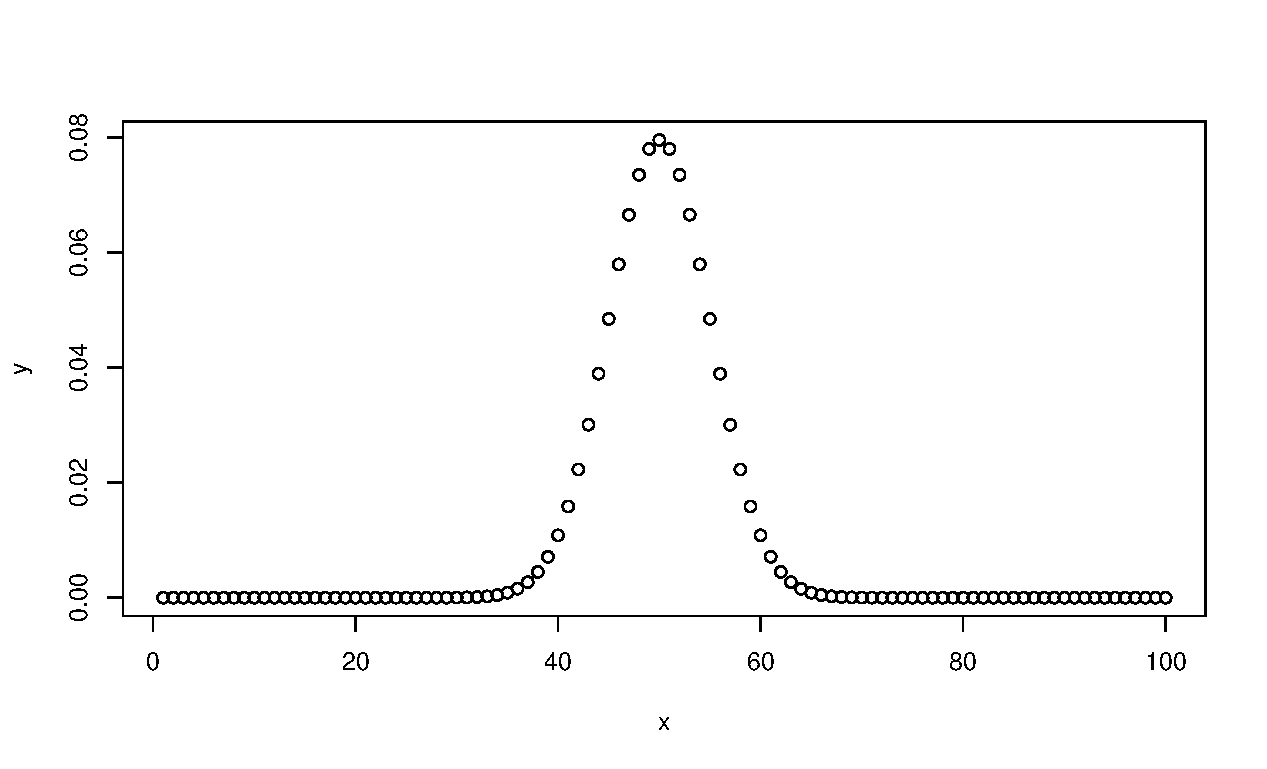
\includegraphics[width=1\textwidth]{binom}
    \end{minipage}\\
    \hline
  \end{tabular}
  \caption{Code and Plot side by side}
  \label{table:3}
\end{table}


% Inline Code
\section{Inline Code usage}

Using inline code in LaTeX is possible using \verb|\verb| command.
It would be repoduced similarly, as a Inline code element.
\begin{verbatim}
\verb|x <- 1:100|
\end{verbatim}
will be represented as \verb|x <- 1:100| in Inline format.

\section{Code chunks using Schunk}
Code chunks within an \verb|Schunk| environment to demonstrate Input/Output

\begin{Schunk}
Input :
\begin{Sinput}
print("Hello world")
\end{Sinput}
Output :
\begin{Soutput}
[1] "hello world"
\end{Soutput}
\end{Schunk}

Similar arrangement can be had for Plots as well using figure environnment.

\begin{Schunk}
Input :
\begin{Sinput}
x <- 1:100
y <- dbinom(x,100,prob = 0.5)
plot(x,y)
\end{Sinput}
Output :\\
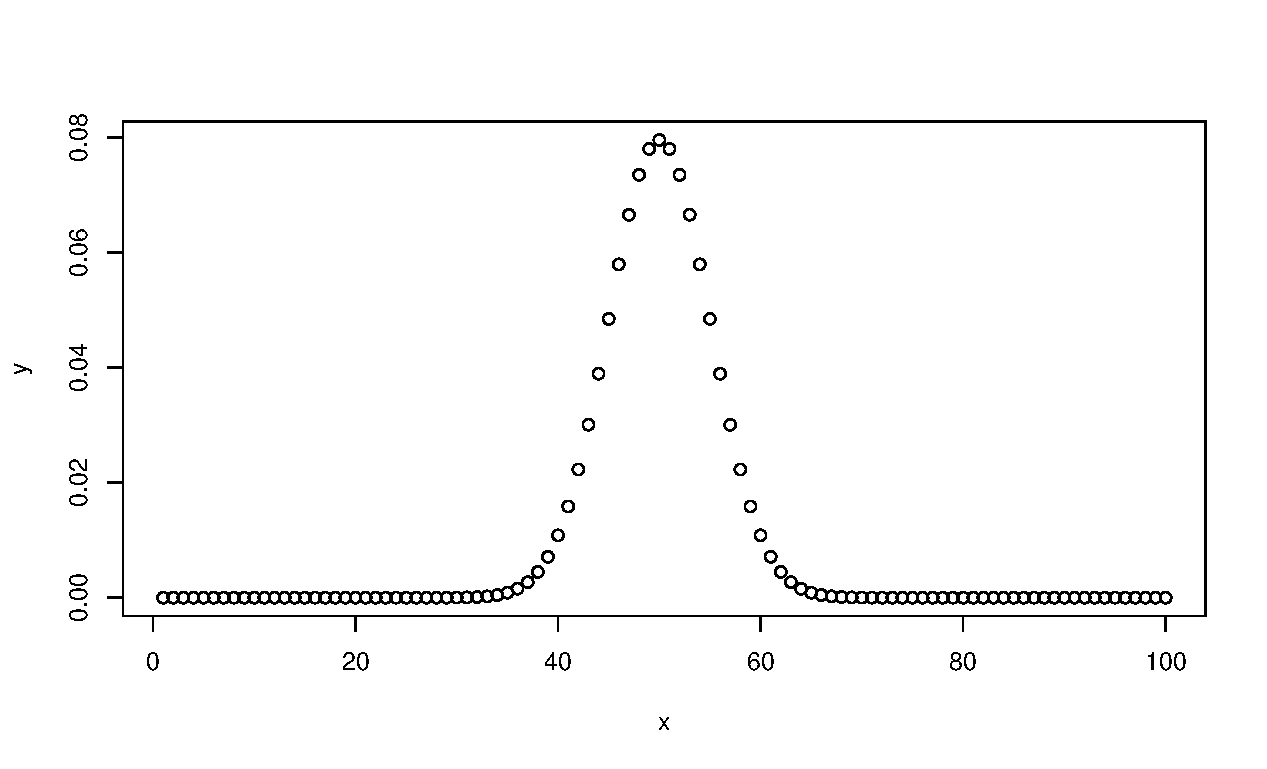
\includegraphics[width=0.5\textwidth]{binom}
\end{Schunk}


\section{Summary}

In summary the \CRANpkg{texor} package supports:
\begin{itemize}
\item Almost all code environments in RJournal.
\item Code Highlight for R language.
\item Inline Code.
\item Code in different environments like tables/figures.
\end{itemize}



\begin{thebibliography}{2}
    \providecommand{\natexlab}[1]{#1}
    \providecommand{\url}[1]{\texttt{#1}}
    \expandafter\ifx\csname urlstyle\endcsname\relax
      \providecommand{\doi}[1]{doi: #1}\else
      \providecommand{\doi}{doi: \begingroup \urlstyle{rm}\Url}\fi

\bibitem[Krewinkel, Lucero (2023)]{pandoc}
A.~ Krewinkel and A.~ Lucero
\newblock pandoc 3.0 Release notes
\newblock \emph{pandoc} \penalty0 2023
\newblock URL \url{https://pandoc.org/releases.html#pandoc-3.0-2023-01-18}

\bibitem[Fairbairns, Duggan, Schöpf, Eijkhout (2011)]{moreverb}
R.~ Fairbairns, A.~ Duggan, R.~ Schöpf and V.~ Eijkhout
\newblock The moreverb package documentation
\newblock \emph{CTAN} \penalty0 2011
\newblock URL \url{https://mirror.niser.ac.in/ctan/macros/latex/contrib/moreverb/moreverb.pdf}

\end{thebibliography}


\address{%
Abhishek Ulayil\\
Student, Institute of Actuaries of India\\%
Mumbai, India\\
ORCiD: 0009-0000-6935-8690\\
}
